%(BEGIN_QUESTION)
% Copyright 2008, Tony R. Kuphaldt, released under the Creative Commons Attribution License (v 1.0)
% This means you may do almost anything with this work of mine, so long as you give me proper credit

{\it HART}-protokollen var et tidlig forsøk på en digital kommunikasjonsstandard for feltinstrumenter, utviklet som en utvidelse av den etablerte 4--20 mA DC-standarden. Hovedideen er at seriell digitaldata kodes som høyfrekvente AC-signaler superponert på DC-spenningen i en 4--20 mA-sløyfe:

$$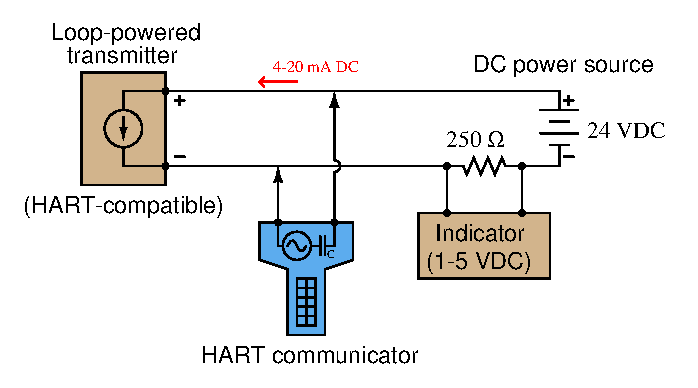
\includegraphics[width=15.5cm]{i00400x01.eps}$$

En mikroprosessor i den sløyfedrevne transmitteren detekterer digitaldata fra HART-kommunikatoren som små AC-pulser over transmitterterminalene. Transmitteren kan på sin side sende digitaldata tilbake i samme format, som kommunikatøren leser som AC-pulser over sine terminaler.

Bruk superposisjonsteoremet på kretsen, og vis hvordan kretsen ``ser ut'' for AC-signalene mellom transmitter og kommunikator, og hvordan den ``ser ut'' for DC-signalene mellom transmitter og indikator.

\vskip 10pt

Angi også hvor i kretsen kommunikatoren kan kobles inn og fortsatt kunne ``snakke'' med smartinstrumentet. Hvilke fordeler gir det å kunne koble kommunikatoren på ulike punkter?

\underbar{file i00400}
%(END_QUESTION)





%(BEGIN_ANSWER)

\noindent
{\bf Krets slik den fremstår for AC (HART)-signaler sendt av kommunikatoren:}

$$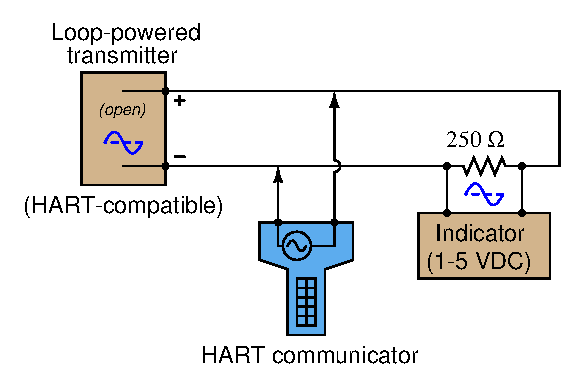
\includegraphics[width=15.5cm]{i00400x02.eps}$$

\vskip 10pt

\noindent
{\bf Krets slik den fremstår for DC (4--20 mA)-signaler:}

$$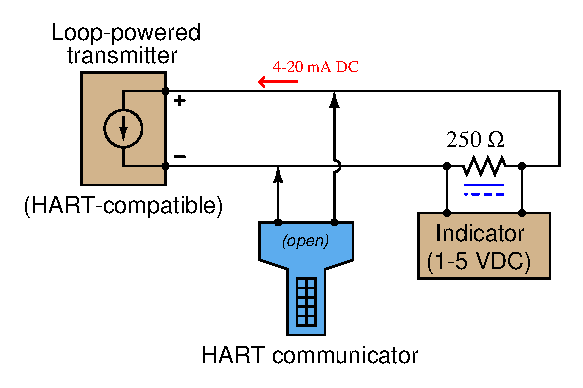
\includegraphics[width=15.5cm]{i00400x03.eps}$$

\vskip 10pt

Kommunikatoren kan kobles {\it hvor som helst} som gir parallellkobling med transmitterterminalene, fra transmitteren i felt og helt tilbake til kontrollpanelet der indikatoren står.

\vskip 10pt

Utfordringsspørsmål: En HART-kommunikator kan også kommunisere med smartinstrumentet når den kobles direkte parallelt med 250 $\Omega$ sløyfemotstanden, selv om dette teknisk sett ikke er direkte parallelt med transmitterterminalene. Forklar hvorfor det fungerer.

%(END_ANSWER)





%(BEGIN_NOTES)

Merk at transmitteren ikke er en ekte effektkilde slik strømkildesymbolet kan antyde. Den fungerer som strøm{\it regulator}. Den reelle effektkilden er 24 V DC-batteriet. Likevel er det gyldig å ``fjerne'' 24 V-kilden ved superposisjonsanalyse for å synliggjøre signalveiene.

Merk også at HART-signalet legger seg over 250 ohm-motstanden like mye som over transmitteren. Dette betyr at HART-kommunikatoren i prinsippet kan påvirke prosesssignalet som indikator/regulator mottar. I de fleste tilfeller hindrer lavpassfiltrering i instrumentene problemer, men ikke alltid. Det er observert regulatorer med fluktuerende PV-visning mens HART-kommunikator ``snakker'' på sløyfen. Derfor kan det være lurt å sette regulatoren i {\it manuell} modus under digital kommunikasjon med transmitter.

\vskip 10pt

Det er viktig at studenter forstår at HART-kommunikator kan kobles {\it hvor som helst} i sløyfen som gir parallellforbindelse mot transmitterterminalene. Denne fleksibiliteten gjør at teknikere kan sjekke parametere og endre område på felttransmittere fra kontrollrommet. Det betyr også at HART-kompatible kontrollsystemer (som mange DCS-er) kan lese smartparametere uten ekstra ledningspar utover eksisterende 4--20 mA-kabel.

Parallellkobling over 250 $\Omega$-motstanden er mulig fordi DC-kilden ``ses'' av HART-signalene fra både kommunikator og transmitter som en kortslutning.

%INDEX% Fieldbus, HART: analysis of 4-20 mA / HART transmitter circuit using Superposition Theorem

%(END_NOTES)
